\documentclass[12pt,twoside]{article}

\textwidth 17cm \textheight 25cm \evensidemargin 0cm
\oddsidemargin 0cm \topmargin -2cm
\parindent 0pt
%\parskip \bigskipamount

\usepackage{graphicx}
\usepackage[dutch]{babel}
\usepackage{amssymb,amsthm,amsmath}
%\usepackage{dot2texi}
\usepackage[utf8]{inputenc}
\usepackage{nopageno}
\usepackage{pdfpages}
\usepackage{enumerate}
\usepackage{caption}
\usepackage{wrapfig}
\usepackage{pgf,tikz,pgfplots}
\pgfplotsset{compat=1.15}
\usepackage{color}
\usetikzlibrary{arrows}
\usetikzlibrary{patterns}
\usepackage{fancyhdr}
\pagestyle{fancy}
\usepackage[version=3]{mhchem}
\usepackage{multicol}
\usepackage{fix-cm}
\usepackage{setspace}
\usepackage{mhchem}
\usepackage{xhfill}
\usepackage{parskip}
\usepackage{cancel}
\usepackage{mdframed}
\usepackage{url}
\usepackage{mathtools}
\usepackage{changepage}

\newcommand{\todo}[1]{{\color{red} TODO: #1}}

\newcommand{\degree}{\ensuremath{^\circ}}
\newcommand\rad{\qopname\relax o{\mathrm{rad}}}

\newcommand\ggd{\qopname\relax o{\mathrm{ggd}}}

\pgfmathdeclarefunction{gauss}{2}{%
  \pgfmathparse{1/(#2*sqrt(2*pi))*exp(-((x-#1)^2)/(2*#2^2))}%
}

\def\LRA{\Leftrightarrow}

\newcommand{\zrmbox}{\framebox{\phantom{EXE}}\phantom{X}}
\newcommand{\zrm}[1]{\framebox{#1}}

% environment oefening:
% houdt een teller bij die de oefeningen nummert, probeert ook de oefening op één pagina te houden
\newcounter{noefening}
\setcounter{noefening}{0}
\newenvironment{oefening}
{
  \stepcounter{noefening}
  \pagebreak[0]
  \begin{minipage}{\textwidth}
  \vspace*{0.7cm}{\large\bf Oefening \arabic{noefening}}
}{%
  \end{minipage}
}

\usepackage{calc}

% vraag
\reversemarginpar
\newcounter{punten}
\setcounter{punten}{0}
\newcounter{nvraag}
\setcounter{nvraag}{1}
\newlength{\puntwidth}
\newlength{\boxwidth}
\newcommand{\vraag}[1]{
\settowidth{\puntwidth}{\Large{#1}}
\setlength{\boxwidth}{1.5cm}
\addtolength{\boxwidth}{-\puntwidth}
{\large\bf Vraag \arabic{nvraag} \addtocounter{nvraag}{1}}\vspace*{-0.5cm}
{\marginpar{\color{lightgray}\fbox{\parbox{1.5cm}{\vspace*{1cm}\hspace*{\boxwidth}{\Large{#1}}}}}
\vspace*{0.5cm}}
\addtocounter{punten}{#1}}

% arulefill
\def\arulefill{\leavevmode{\xrfill[-5pt]{0.3pt}[lightgray]\endgraf}\vspace*{0.2cm}}

% \arules{n}
\newcommand{\arules}[1]{
\color{lightgray}
%\vspace*{0.05cm}
\foreach \n in {1,...,#1}{
  \vspace*{0.75cm}
  \hrule height 0.3pt\hfill
}\color{black}\vspace*{0.2cm}}

% \arule{x}
\newcommand{\arule}[1]{
\color{lightgray}{\raisebox{-0.1cm}{\rule[-0.05cm]{#1}{0.3pt}}}\color{black}
}

% \abox{y}
\newcommand{\abox}[1]{
\fbox{
\begin{minipage}{\textwidth- 4\fboxsep}
\hspace*{\textwidth}\vspace{#1}
\end{minipage}
}
}

\newcommand{\ruitjes}[1]{
\definecolor{cqcqcq}{rgb}{0.85,0.85,0.85}
\hspace*{-2.5cm}
\begin{tikzpicture}[scale=1.04,line cap=round,line join=round,>=triangle 45,x=1.0cm,y=1.0cm]
\draw [color=cqcqcq, xstep=0.5cm, ystep=0.5cm] (0,-#1) grid (20.5,0);
\end{tikzpicture}
}


\newcommand{\assenstelsel}[5][1]{
\definecolor{cqcqcq}{rgb}{0.65,0.65,0.65}
\begin{tikzpicture}[line cap=round,line join=round,>=triangle 45,x=#1cm,y=#1cm]
\draw [color=cqcqcq,dash pattern=on 1pt off 1pt, xstep=1.0cm,ystep=1.0cm] (#2,#4) grid (#3,#5);
\draw[->,color=black] (#2,0) -- (#3,0);
%\draw[shift={(1,0)},color=black] (0pt,2pt) -- (0pt,-2pt) node[below] {\footnotesize $1$};
%\draw[color=black] (#3.25,0.07) node [anchor=south west] {$x$};
\draw[->,color=black] (0,#4) -- (0,#5);
%\draw[shift={(0,1)},color=black] (2pt,0pt) -- (-2pt,0pt) node[left] {\footnotesize $1$};
\draw[color=black] (0.09,#5.25) node [anchor=west] {\phantom{$y$}};
%\draw[color=black] (0pt,-10pt) node[right] {\footnotesize $0$};
\end{tikzpicture}
}

\newcommand{\getallenas}[3][1]{
\definecolor{cqcqcq}{rgb}{0.65,0.65,0.65}
\begin{tikzpicture}[scale=#1,line cap=round,line join=round,>=triangle 45,x=1.0cm,y=1.0cm]
\draw [color=cqcqcq,dash pattern=on 1pt off 1pt, xstep=1.0cm,ystep=1.0cm] (#2,-0.2) grid (#3,0.2);
\draw[->,color=black] (#2.25,0) -- (#3.5,0);
\draw[shift={(0,0)},color=black] (0pt,2pt) -- (0pt,-2pt) node[below] {\footnotesize $0$};
\draw[shift={(1,0)},color=black] (0pt,2pt) -- (0pt,-2pt) node[below] {\footnotesize $1$};
\draw[color=black] (#3.25,0.07) node [anchor=south west] {$\mathbb{R}$};
\end{tikzpicture}
}

\newcommand{\visgraad}[1]{\begin{tabular}{p{0.5cm}|p{#1}}&\\\hline\\\end{tabular}}

\newcommand{\tekenschema}[2]{\begin{tabular}{p{0.5cm}|p{#1}}&\\\hline\\[#2]\end{tabular}}

% schema van Horner
\newcommand{\schemahorner}{
\begin{tabular}{p{0.5cm}|p{7cm}}
&\\[1.5cm]
\hline\\
\end{tabular}}

% geef tabular iets meer ruimte
\setlength{\tabcolsep}{14pt}
\renewcommand{\arraystretch}{1.5}

\newcommand{\toets}[3]{
\thispagestyle{plain}
\vspace*{-2.5cm}
\begin{tikzpicture}[remember picture, overlay]
    \node [shift={(15.25 cm,-1.6cm)}] {%
        \includegraphics[width=1.8cm]{/home/ppareit/kaa1415/logokaavelgem.png}%
    };%
\end{tikzpicture}

\begin{tabular}{|llc|c|}
\hline
\vspace*{-0.5cm}
&&&\\
Naam & \arule{4cm} & {\Large\bf KA AVELGEM} & \\
\vspace*{-0.75cm}
&&&\\
Klas & \arule{4cm} & {\Large\bf 20...-...-...} & \\
\hline
\vspace*{-0.75cm}
&&&\\
Toets & {\bf #2} & {\large\bf #1} & Beoordeling\\
\vspace*{-0.75cm}
&&&\\
Onderwerp & \multicolumn{2}{l|}{\bf #3} &\\
\hline
\end{tabular}
}

\newcommand{\oefeningen}[1]{

\fancyhead[LE, RO]{\vspace{0.5cm} #1}
%\thispagestyle{plain}

{\bf \Large \centering Oefeningen: #1}

}

\raggedbottom

\newcommand\vl{\qopname\relax o{\mathrm{vl}}}

\newcommand\dom{\qopname\relax o{\mathrm{dom}}}
\newcommand\ber{\qopname\relax o{\mathrm{ber}}}

\newcommand\mC{\qopname\relax o{\mathrm{mC}}}
\newcommand\uC{\qopname\relax o{\mathrm{{\mu}C}}}
\newcommand\C{\qopname\relax o{\mathrm{C}}}

\newcommand\W{\qopname\relax o{\mathrm{W}}}
\newcommand\kW{\qopname\relax o{\mathrm{kW}}}
\newcommand\kWh{\qopname\relax o{\mathrm{kWh}}}


\newcommand\V{\qopname\relax o{\mathrm{V}}}
\newcommand\ohm{\qopname\relax o{\mathrm{\Omega}}}
\newcommand\kohm{\qopname\relax o{\mathrm{k\Omega}}}


\newcommand\N{\qopname\relax o{\mathrm{N}}}

\newcommand\Nperkg{\qopname\relax o{\mathrm{N/kg}}}

\newcommand\Nperm{\qopname\relax o{\mathrm{N/m}}}

\newcommand\gpermol{\qopname\relax o{\mathrm{g/mol}}}


\newcommand\kgperm{\qopname\relax o{\mathrm{kg/m}}}
\newcommand\kgperdm{\qopname\relax o{\mathrm{kg/dm}}}
\newcommand\gpercm{\qopname\relax o{\mathrm{g/cm}}}
\newcommand\gperml{\qopname\relax o{\mathrm{g/ml}}}


\newcommand{\mA}{\;\mbox{mA}}
\newcommand{\A}{\;\mbox{A}}
\newcommand{\MA}{\;\mbox{MA}}

\newcommand{\us}{\;\mu\mbox{s}}
\newcommand\s{\qopname\relax o{\mathrm{s}}}

\newcommand\h{\qopname\relax o{\mathrm{h}}}

\newcommand{\kmperh}{\;\mbox{km/h}}
\newcommand{\mpers}{\;\mbox{m/s}}
\newcommand{\kmpermin}{\;\mbox{km/min}}
\newcommand{\kmpers}{\;\mbox{km/s}}

\newcommand{\mph}{\;\mbox{mph}}

\newcommand{\Hz}{\;\mbox{Hz}}

\newcommand\Gm{\qopname\relax o{\mathrm{Gm}}}
\newcommand\Mm{\qopname\relax o{\mathrm{Mm}}}
\newcommand\km{\qopname\relax o{\mathrm{km}}}
\newcommand\hm{\qopname\relax o{\mathrm{hm}}}
\newcommand\dam{\qopname\relax o{\mathrm{dam}}}
\newcommand\m{\qopname\relax o{\mathrm{m}}}
\newcommand\dm{\qopname\relax o{\mathrm{dm}}}
\newcommand\cm{\qopname\relax o{\mathrm{cm}}}
\newcommand\mm{\qopname\relax o{\mathrm{mm}}}
\newcommand\um{\qopname\relax o{\mathrm{{\mu}m}}}
\newcommand\nm{\qopname\relax o{\mathrm{nm}}}


\newcommand\Gg{\qopname\relax o{\mathrm{Gg}}}
\newcommand\Mg{\qopname\relax o{\mathrm{Mg}}}
\newcommand\kg{\qopname\relax o{\mathrm{kg}}}
\newcommand\hg{\qopname\relax o{\mathrm{hg}}}
\renewcommand\dag{\qopname\relax o{\mathrm{dag}}}
\newcommand\g{\qopname\relax o{\mathrm{g}}}
\newcommand\dg{\qopname\relax o{\mathrm{dg}}}
\newcommand\cg{\qopname\relax o{\mathrm{cg}}}
\newcommand\mg{\qopname\relax o{\mathrm{mg}}}
\newcommand\ug{\qopname\relax o{\mathrm{{\mu}g}}}
\renewcommand\ng{\qopname\relax o{\mathrm{ng}}}

\newcommand\ton{\qopname\relax o{\mathrm{ton}}}

\newcommand\Gl{\qopname\relax o{\mathrm{Gl}}}
\newcommand\Ml{\qopname\relax o{\mathrm{Ml}}}
\newcommand\kl{\qopname\relax o{\mathrm{kl}}}
\newcommand\hl{\qopname\relax o{\mathrm{hl}}}
\newcommand\dal{\qopname\relax o{\mathrm{dal}}}
\renewcommand\l{\qopname\relax o{\mathrm{l}}}
\newcommand\dl{\qopname\relax o{\mathrm{dl}}}
\newcommand\cl{\qopname\relax o{\mathrm{cl}}}
\newcommand\ml{\qopname\relax o{\mathrm{ml}}}
\newcommand\ul{\qopname\relax o{\mathrm{{\mu}l}}}
\newcommand\nl{\qopname\relax o{\mathrm{nl}}}

\newcommand\MJ{\qopname\relax o{\mathrm{MJ}}}
\newcommand\kJ{\qopname\relax o{\mathrm{kJ}}}
\newcommand\J{\qopname\relax o{\mathrm{J}}}

\newcommand\T{\qopname\relax o{\mathrm{T}}}
\newcommand\uT{\qopname\relax o{\mathrm{{\mu}T}}}

\newcommand\grC{\qopname\relax o{\mathrm{{\degree}C}}}

\newcommand\K{\qopname\relax o{\mathrm{K}}}
\newcommand\calperK{\qopname\relax o{\mathrm{cal/K}}}

\newcommand\hPa{\qopname\relax o{\mathrm{hPa}}}
\newcommand\Pa{\qopname\relax o{\mathrm{Pa}}}

\newcommand\dB{\qopname\relax o{\mathrm{dB}}}

\newcommand\Var{\qopname\relax o{\mathrm{Var}}}

\newcommand{\EE}[1]{\cdot 10^{#1}}

\onehalfspacing

%\setlength{\headsep}{0cm}

\newenvironment{exlist}[1] %
{ \begin{multicols}{#1}
  \begin{enumerate}[(a)]
    \setlength{\itemsep}{0.5em} }
{ \end{enumerate}
  \end{multicols} }




%\usepackage{pgfplots}

%\renewcommand{\rmdefault}{phv} % Arial
%\renewcommand{\sfdefault}{phv} % Arial

\newcommand{\dice}[1]{
\begin{tikzpicture}[x=1em,y=1em,radius=0.1]
  \draw[rounded corners=1] (0,0) rectangle (1,1);
  \ifodd#1
    \fill (0.5,0.5) circle;
  \fi
  \ifnum#1>1
    \fill (0.2,0.2) circle;
    \fill (0.8,0.8) circle;
   \ifnum#1>3
     \fill (0.2,0.8) circle;
     \fill (0.8,0.2) circle;
    \ifnum#1>5
      \fill (0.8,0.5) circle;
      \fill (0.2,0.5) circle;
    \fi
  \fi
\fi
\end{tikzpicture}
}

\begin{document}

\thispagestyle{empty}
\begin{center}
  \begin{mdframed}
  \centering
  \fontsize{40}{60}\selectfont Combinatieleer
  \end{mdframed}
  \vfill
%  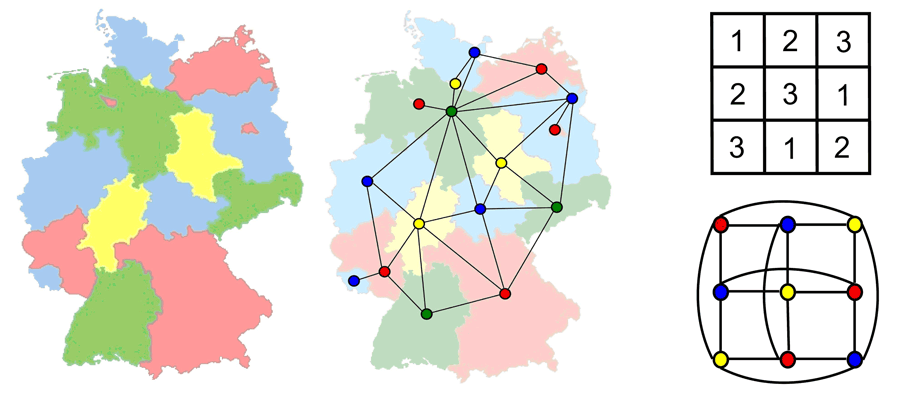
\includegraphics[width=\textwidth]{anewkindofcounting}
  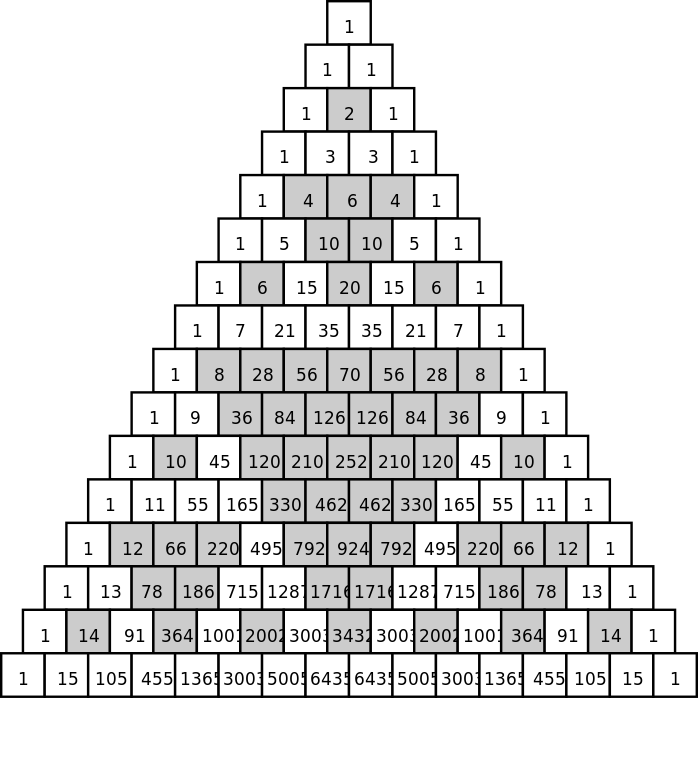
\includegraphics[width=0.8\textwidth]{PascalWithEvenNumbers}
  \vfill
\end{center}
\subsection*{Doelstellingen}
{\singlespacing
Je kan \hfill  {\scriptsize(LP 2006-059, LI 2.1)}
\begin{itemize}
  \itemsep0em
  \item telproblemen oplossen waarbij volgorde en herhaling al dan niet van belang zijn.
  \item eigenschappen in verband met de binomiaalgetallen bewijzen en gebruiken om de driehoek van Pascal op
te stellen. (V)
  \item de formule van het binomium van Newton opstellen en gebruiken. (V)
\end{itemize}}
%\subsection*{Algemene vaardigheden en attitudes}
%{\singlespacing
%Je \hfill {\scriptsize(LP 2006/059, ET1, ET9, ET11)}
%\begin{itemize}
%  \itemsep0em
%  \item begrijpt en gebruikt wiskundetaal.
%  \item gebruikt kennis, inzicht en vaardigheden die je verwerft in de wiskunde bij het verkennen, vertolken en verklaren van problemen uit de realiteit.
%  \item ontwikkelt zelfregulatie met betrekking tot het verwerven en verwerken van wiskundige informatie en het oplossen van problemen
%\end{itemize}
%}

\thispagestyle{empty}
\mbox{}
\newpage
\clearpage
\thispagestyle{empty}
\mbox{}
\newpage
\clearpage
\pagenumbering{arabic} 

\fancyhead[RO,LE]{Combinatieleer}
\fancyhead[RE,LO]{}

\section{Inleiding}

We beginnen aan een hoofdstuk die vaak combinatoriek of combinatieleer wordt genoemd. Wij zullen voornamelijk problemen bespreken waarbij we het aantal mogelijkheden of het aantal objecten van een verzameling moeten tellen. We spreken dan ook van {\bf telproblemen}.

\section{Productregel}

\subsubsection*{Voorbeeld}

Deze zomer ben ik eens op restaurant geweest en daar hing volgende menu:

\begin{mdframed}
\begin{itemize}
  \item Voorgerechten:
  \begin{itemize}
    \item Garnaalkroketten
    \item Gerookte zalm
  \end{itemize}
  \item Hoofdgerechten:
  \begin{itemize}
    \item Lasagne
    \item Pasta met kip
    \item Biefstuk met peper-roomsaus
  \end{itemize}
  \item desserts:
  \begin{itemize}
    \item Appeltaart
    \item Sorbet
  \end{itemize}
\end{itemize}
\end{mdframed}

Ik had uiteraard veel honger en bestelde één voorgerecht, één hoofdgerecht en één dessert.

We wensen dus een maaltijd samen te stellen, we nemen dus een {\bf samengestelde beslissing} gebaseerd op verschillende onafhankelijke deelbeslissingen in een willekeurige volgorde. Logisch is dat we eerst een voorgerecht kiezen, dan een hoofdgerecht en als laatste een dessert. Onze menu zal echter niet wijzigen als we eerst een beslissing nemen over het dessert en daarna over het voorgerecht en het hoofdgerecht.

De vraag is nu:\\
{\em Op hoeveel manieren kan ik mijn menu samenstellen?}

Om zeker te zijn dat we de telling juist doen zullen we het probleem grafisch gaan voorstellen. We kunnen dit op drie manieren doen, met een boomdiagram, met een wegendiagram of met een vaasmodel. Elke voorstellingswijze heeft voor- en nadelen.

\subsection{Boomdiagram}

\hspace*{2cm} Voorgerecht \hfill Hoofdgerecht \hfill Dessert \hspace*{2cm}

\vspace*{8cm}
start
\vspace*{8cm}

In een wiskundige boom worden de lijntjes de {\bf takken} genoemd. De takken komen steeds samen in de {\bf knopen}. De knoop waar begonnen wordt noemen we de {\bf wortel} en het eindpunten van de boom worden de {\bf bladen} genoemd.

\begin{oefening}
Hoeveel mogelijke menu's kunnen we kiezen en wat hebben we moeten tellen op de boom?
\arules{2}
\end{oefening}

\begin{oefening}
Neem eens de beslissingen in een andere volgorde, namelijk kies eerst een dessert, dan een voorgerecht en dan pas het hoofdgerecht. Teken de boom. Krijg je dezelfde boom? Krijg hetzelfde aantal mogelijkheden?
\end{oefening}

\subsection{Wegendiagram}

Een boomdiagram heeft als voornaamste nadeel dat deze heel snel heel groot wordt. Als je nu eens kijkt naar de boom, dan merk je dat er per beslissing evenveel takken vertrekken uit een knoop. Laat je de vertrekkende takken dus toekomen in éénzelfde knoop dan wordt de figuur veel compacter:

\hspace*{2cm} Voorgerecht \hfill Hoofdgerecht \hfill Dessert \hspace*{2cm}

\vspace*{3cm}
start
\vspace*{3cm}

Het tellen wordt nu moeilijker, we bekijken de verschillende deelbeslissingen apart.
\begin{itemize}
  \item Voor je voorgerecht neem je een éérste beslissing, je hebt \arule{2cm} keuzes.
  \item Voor je hoofdgerecht neem je een tweede beslissing, je hebt \arule{2cm} keuzes.
  \item Voor je dessert neem je een derde beslissing, je hebt \arule{2cm} keuzes.
\end{itemize}

We weten nu dat het aantal mogelijke menu's via de methode van het wegendiagram evenveel moet zijn als via de methode van het boomdiagram.

\begin{oefening}
Hoeveel mogelijke menu's kunnen we kiezen en hoe berekenen we dit?
\arules{2}
\end{oefening}

\subsection{Vaasmodel}

We kunnen het probleem ook voorstellen met behulp van vazen. Voor elke beslissing die we moeten nemen, nemen we een vaas met in deze vaas evenveel balletjes als het aantal keuzen die deze beslissing heeft.

\hspace*{2cm} Voorgerecht \hfill Hoofdgerecht \hfill Dessert \hspace*{2cm}

\vspace*{4cm}

\begin{oefening}
Neem nu uit elke vaas een balletje, welk gerecht heb je samengesteld? Hoeveel andere gerechten kan je nog samenstellen?
\arules{2}
\end{oefening}

\subsection{Productregel}

Om een ander voorbeeld te bekijken, we wensen ons aan te kleden en we hebben keuze uit 3 truien en 2 broeken, dan kunnen we ons op $3\cdot 2 = 6$ manieren kleden. Je kiest eerst een trui wat op 3 manieren kan, en bij elk van de drie keuzes van truien heb je twee mogelijkheden om een broek te kiezen. Dit soort telproblemen kunnen we oplossen met wat we de productregel noemen:

\paragraph*{Productregel}
\begin{mdframed}
Als een telprobleem bestaat uit $r$ onafhankelijke deelbeslissingen waarbij er voor de deelbeslissingen respectievelijk $n_1, n_2, \ldots, n_r$ mogelijkheden zijn, dan zijn er in het totaal
$$n_1\cdot n_2\cdot \ldots \cdot n_r$$
mogelijkheden.
\end{mdframed}

\pagebreak
\subsection{Oefeningen}\vspace*{-1cm}

\begin{oefening}
In een sportclub stelt men T-shirts, shorts en kousen ter beschikking voor de spelers. Er zijn oranje, witte, blauwe, rode en groene T-shirts. De shorts zijn zwart, blauw of wit. De kousen zijn wit met een blauwe boord ofwel effen wit. Er zijn dus heel wat outfits voor de spelers mogelijk.

Teken het boomdiagram en het wegendiagram dat met de gegevens correspondeert. Hoeveel mogelijke outfits zijn er voor de spelers?
\end{oefening}

\begin{oefening}
In de kantine van een fabriek staat een machine voor warme dranken. De leverancier wil gewone koffie, espresso en thee aanbieden, met of zonder melk, zonder, met weinig of met veel suiker. Hij heeft voor elke mogelijkheid een knop voorzien.

Teken het wegendiagram. Bepaal het aantal knoppen op de machine.
\end{oefening}

\begin{oefening}
Vanaf de ingang van de zoo zijn er drie paden naar het dolfinarium. Van het dolfinarium naar de apen zijn er 4 paden. Van de apen naar de pinguïns zijn er twee paden. En van de pinguïns naar de tijgers zijn er drie paden.

Ik wil naar de show van de dolfijnen gaan kijken. Als ik van de ingang naar de dolfijnen wandel zie ik de uren van de shows geafficheerd staan en merk ik dat ik nog ruim voldoende tijd heb om eerst een bezoekje te brengen aan de apen, de pinguïns en de tijgers.

\begin{enumerate}[(a)]
  \item Hoeveel verschillende wandelingen zijn er mogelijk van de ingang tot de tijgers?
  \item Bij de tijgers pauzeer ik even tot het tijd is om terug te keren naar het dolfinarium voor de show. Ik kies een wandeling terug via de pinguïns en de apen, maar wil een pad dat ik op de heenweg nam geen tweede keer bewandelen.
  
  Schets en wegendiagram van deze tweede wandeling. Hoeveel wandelingen zijn er nu mogelijk van de tijgers naar de dolfijnen?
\end{enumerate}

\begin{center}
  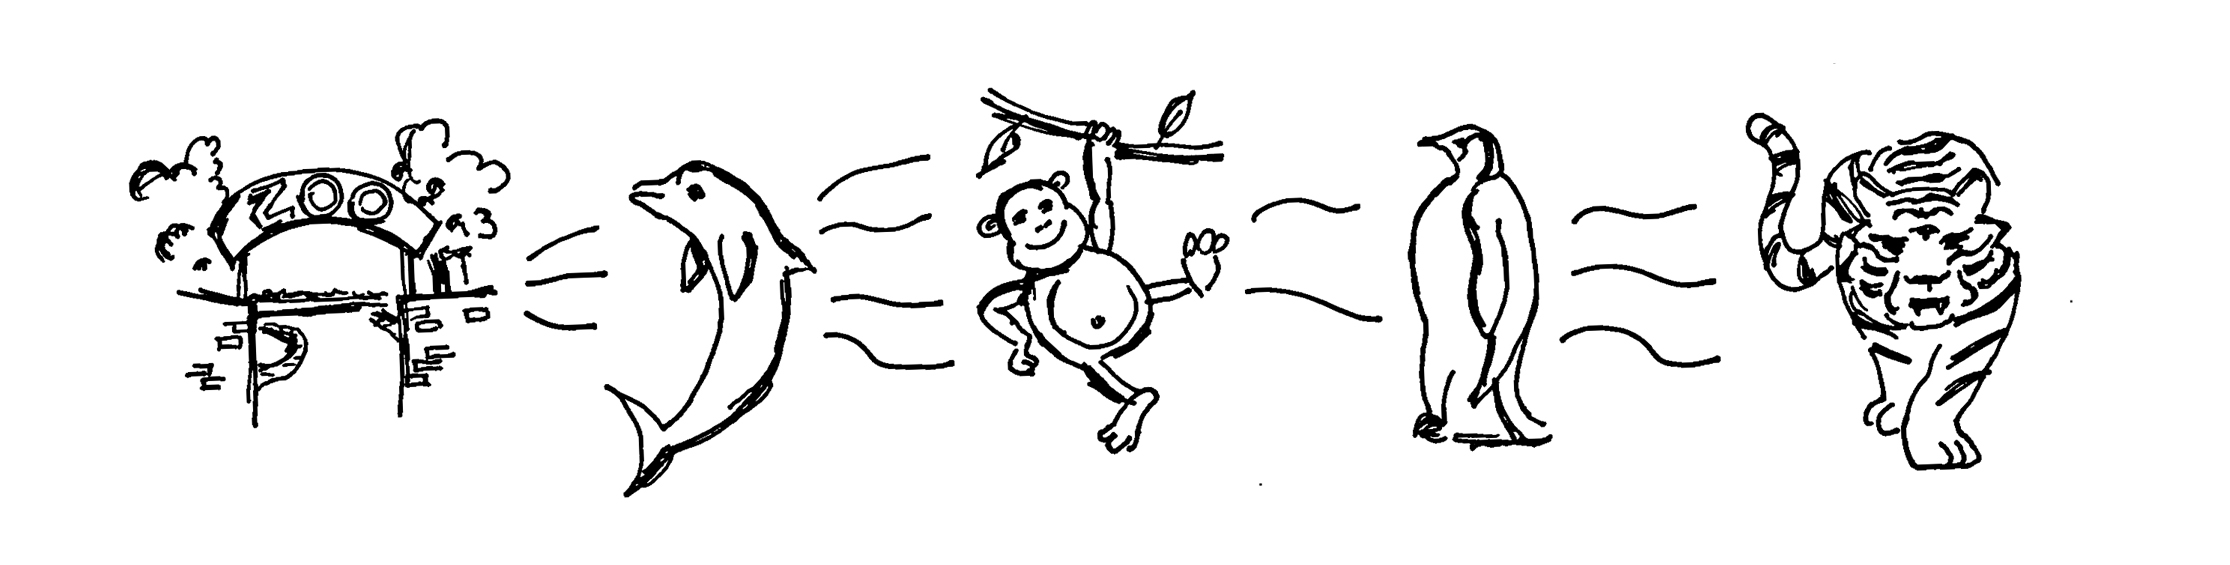
\includegraphics[width=\textwidth]{zoodieren}
\end{center}
\end{oefening}

\vspace*{-1cm}
\begin{oefening}
Los volgende problemen op met behulp van een boomdiagram.
\begin{enumerate}[(a)]
  \item Hoeveel natuurlijke getallen zijn er met drie cijfers, te kiezen uit 2, 3, 5 en 7?
  \item Hoeveel natuurlijke getallen zijn er met drie {\em verschillende} cijfers, te kiezen uit 2, 3, 5 en 7?
  \item Hoeveel natuurlijke getallen van drie verschillende cijfers, te kiezen uit 2, 3, 5 en 7, beginnen met een 5?
  \item Hoeveel natuurlijke getallen van drie verschillende cijfers, te kiezen uit 2, 3, 5 en 7, eindigen op een 5?
\end{enumerate}
\end{oefening}

\section{Somregel}

\subsection{Somregel met dubbele telling}

\subsubsection*{Voorbeeld}

Vorige winter ben ik met een aantal vrienden uit het middelbaar iets gaan eten. We bestelden allemaal een hoofdgerecht en er werden 11 voorgerechten en 7 desserts besteld. Met vijf aten we zowel een voorgerecht als een dessert. Met hoeveel waren we?

\begin{oefening}
Maak een venndiagram van de verzameling van de voorgerecht-eters en de nagerecht-eters. Leid hieruit het aantal af.
\vspace*{4cm}
\end{oefening}

Als je dus het aantal personen met een dessert het aantal personen met een voorgerecht optelt dan tel je de personen die een voorgerecht en een dessert hebben gegeten dubbel. Je kan dit compenseren door door éénmaal de personen die je dubbel hebt geteld er weer van af te trekken.

\paragraph*{Somregel}
\begin{mdframed}
Voor het aantal elementen van de unie van twee verzamelingen $A$ en $B$ geldt:
$$\#(A\cup B) = \#A + \#B - \#(A\cap B)$$
waarin
\begin{itemize}
  \item $\#A$ staat voor het aantal elementen van de verzameling $A$
  \item $A\cup B$ staat voor de unie (vereniging) van de verzamelingen $A$ en $B$, we kunnen dit ook omschrijven als $A$ {\em of} $B$
  \item $A\cap B$ staat voor de doorsnede van de verzamelingen $A$ en $B$, we kunnen dit ook omschrijven als $A$ {\em en} $B$
\end{itemize}
\end{mdframed}

\begin{oefening}
Bepaal met behulp van de somregel het aantal kaarten in een set van 52 kaarten die harten of koning zijn. Gebruik een set kaarten om dit te controleren. Maak ook een het bijhorende venndiagram.
\end{oefening}

\subsection{Somregel van elkaar uitsluitende mogelijkheden}

\subsubsection*{Voorbeeld}

Bepaal het aantal natuurlijke getallen van vier verschillende cijfers die deelbaar zijn door 5.

\begin{oefening}
Geef een goede voorstelling van het getal. Duid ook per cijfer het aantal mogelijkheden aan.
\arules{2}
\end{oefening}

Stel $B=$ de verzameling van alle mogelijke getallen van 4 verschillende cijfers die deelbaar zijn door 5

\begin{oefening}
Hoe herkennen we getallen die deelbaar zijn door vijf? Gebruik deze eigenschap om $B$ te splitsen in een aantal deelverzamelingen. Definieer de deelverzamelingen en teken het bijhorende venndiagram.
\arules{4}
\vspace*{4cm}
\end{oefening}

\begin{oefening}
Wat weten we over de deelverzamelingen?
\arules{1}
\end{oefening}

We zeggen dat de deelverzamelingen elkaar {\bf uitsluitende mogelijkheden} zijn. Dit wil zeggen dat we de somregel kunnen toepassen zonder dat we het aantal elementen in de doorsnede moeten uitrekenen.

\begin{oefening}
\begin{enumerate}[(a)]
  \item Bereken $\#B_1$ met behulp van de productregel.
  \arules{6}
  \item Bereken $\#B_2$ met behulp van de productregel.
  \arules{6}
  \item Bereken nu $\#B$ uit met behulp van de somregel en los het telprobleem op.
  \arules{2}
\end{enumerate}
\end{oefening}

\paragraph*{Somregel voor elkaar uitsluitende mogelijkheden}
\begin{mdframed}
Zijn de twee verzamelingen $A$ en $B$ elkaar uitsluitende mogelijkheden omdat ze geen elementen gemeenschappelijk hebben, dan geldt voor het aantal elementen in hun unie:
$$\#(A\cup B) = \#A + \#B$$
\end{mdframed}

\begin{oefening}
Een club bestaat uit 30 mannelijke en 50 vrouwelijke leden.
\begin{enumerate}[(a)]
  \item Op hoeveel manieren kan men 1 lid kiezen als voorzitter?
  \item Op hoeveel manieren kan men 1 mannelijk en 1 vrouwelijk lid kiezen als bestuurslid?
\end{enumerate}
\end{oefening}

\begin{oefening}
In een bibliotheek zijn 50 wetenschappelijke verhandelingen, 100 detectiveverhalen en 180 romans beschikbaar. Op hoeveel manieren kan men hieruit 1 boek kiezen? Op hoeveel manieren kan iemand een lijstje opstellen met 1 boek van elke soort?
\end{oefening}

\subsection{Praktisch}

\begin{mdframed}
Bij het oplossen van telproblemen tel je als volgt:
\begin{itemize}
  \item Kan je een boomdiagram maken, dan is het aantal mogelijkheden gelijk aan het aantal bladen.
  \item Kan je een wegendiagram maken, dan is het aantal mogelijkheden gelijk aan het product van de keuzes bij elke beslissing.
  \item Kan je een probleem herschrijven met behulp van {\bf EN}, dan gebruik je de productregel.
  \item Kan je een probleem herschrijven met behulp van {\bf OF}, dan gebruik je de somregel.
\end{itemize}
\end{mdframed}

\begin{minipage}{0.7\textwidth}
\begin{oefening}
We moeten de afloop van 10 voetbalwedstrijden voorspellen. Voor elke match zijn er 3 mogelijkheden: winnen, verliezen en gelijkspel. Hoeveel lijstjes met voorspellingen zijn er mogelijk? Hoe groot is het aantal als we zeker weten dat in de eerste wedstrijd de thuisploeg niet verliest?
\end{oefening}
\end{minipage}
\begin{minipage}{0.25\textwidth}
\hfill
  
\includegraphics[width=0.6\textwidth]{voetbal}
\end{minipage}

\begin{oefening}
Voor de samenstelling van je lessenrooster moet je twee keuzevakken kiezen, elk uit een verschillend vakgebied. Er is keuze uit 3 talen, 4 wetenschappelijke vakken en 2 sporten. Hoeveel keuzemogelijkheden heb je?
\end{oefening}

\begin{oefening}
Het letterslot van een kluis bestaat uit een eerste ring met 10 letters, een tweede ring met 8 letters en een derde ring met 6 letters. Om een kluis te openen moet elke ring zo geplaatst worden dat een bepaalde stand inneemt.
\begin{enumerate}[(a)]
  \item Hoeveel lettergroepen moet een inbreker ten hoogste proberen?
  \item Hoeveel zijn er mogelijk als hij weet dat de letter van de eerste ring een E is?
\end{enumerate}
\end{oefening}

\begin{oefening}
Bij een schoolwedstrijd met 2 ploegen, die elk uit 6 deelnemers bestaan, moet elke deelnemer van de ene ploeg tegen elke deelnemer van de andere ploeg 2 partijen spelen. Hoeveel partijen zijn er in totaal?
\end{oefening}

\begin{oefening}
Bij de aankoop van een wagen moeten we kiezen tussen modellen met 2, 3, 4 of 5 deuren. De wagens met 2 of 3 deuren worden afgeleverd met een motor van 1200, 1400, 1600 of 1800 cc en de wagens met 4 of 5 deuren worden afgeleverd met een motor van 1600, 1800 of 2000 cc. Elke wagen is beschikbaar in 8 kleuren, maar voor de versies 1800 en 2000 cc zijn er bovendien nog 4 gemetalliseerde kleuren mogelijk. Voor wagens met een motor van 1200 cc bestaat er maar 1 type banden, wagens met een grotere motor kunnen naar keuze met één van 2 types banden worden uitgerust. Alle versies zijn verkrijgbaar met of zonder radio. Hoeveel mogelijkheden hebben we bij deze aankoop?
\end{oefening}

\begin{oefening}
Je hebt gewonnen op de foor. Je mag twee prijzen kiezen. Je mag kiezen uit drie verschillende tonnen. Je mag geen twee prijzen kiezen uit dezelfde ton. De eerste ton bevat 3 verschillende mp3-spelers. De tweede ton bevat 4 verschillende sleutelhangers. De laatste ton bevat 2 verschillende horloges. Hoeveel mogelijkheden om te kiezen heb je?
\end{oefening}

\begin{oefening}
Konijnenrassen bestaan in drie soorten: dwergkonijnen, gewone konijnen of reuze konijnen. Alle rassen komen voor als zwart, bruin of wit. Het gewone konijn komt ook nog voor in een zwart-bruin-wit gevlekte variant. Naast de rechtopstaande oren die we gewoon zijn van de konijnen komen dwerg en reuze konijnen ook voor met hangoren. Hoeveel mogelijke soorten konijnen bestaan er dan?
\end{oefening}

\begin{oefening}
Met de cijfers $1, 2, 3, \ldots , 8, 9$ worden getallen van 6 verschillende cijfers gevormd:
\begin{enumerate}[(a)]
  \item Hoeveel zulke getallen zijn er?
  \item Hoeveel van deze getallen beginnen met een 1?
  \item Hoeveel van deze getallen beginnen niet met een 5?
  \item Hoeveel van deze getallen beginnen met 55?
  \item Hoeveel van deze getallen bevatten een 4?
  \item Hoeveel van deze getallen bevatten een 3 en een 8?
  \item Hoeveel van deze getallen bevatten geen 3 en geen 8?
\end{enumerate}
\end{oefening}

\begin{oefening}
Ik ben de pincode van mijn GSM vergeten. Ik weet enkel nog dat er geen 5 in komt, maar wel een 4, en dat het allemaal verschillende cijfers waren. Hoeveel keer moet ik ten hoogste proberen om mijn code terug te vinden (in de veronderstelling dat je zoveel mag proberen als je wilt, zonder dat je sim-kaart geblokkeerd wordt)?
\end{oefening}

% \begin{oefening}
% Stel een boomdiagram op voor de natuurlijke getallen, bestaande uit drie verschillende cijfers, die je met 0, 1, 2, 3 en 4 kan vormen. Hoeveel mogelijke getallen zijn er?
% \end{oefening}
% 
% \begin{oefening}
% Hoeveel getallen, gevormd met de cijfers 0, 5, 6 en 8, liggen tussen 5000 en 6000 (deze twee uitersten inbegrepen) als een cijfer geen tweede maal mag gebruikt worden? Verduidelijk je antwoord met een boomdiagram.
% \end{oefening}
% 
% \begin{oefening}
% Je moet een menu opstellen. Hierbij moet er keuze zijn tussen 2 voorgerechten en 3 hoofdgerechten voor de {\em vegetariërs} en 3 voorgerechten en 4 hoofdgerechten voor de {\em alleseters}. Voor {\em iedereen} is er keuze uit 2 desserts. Hoeveel mogelijke menu's kan je samenstellen?
% \end{oefening}


\section{Variaties}

\subsection{Voorbeeld}

Op hoeveel manieren kunnen vier verschillende bollen in zes verschillende vakjes geplaatst worden? In elk vakje mag hoogstens één bol voorkomen.

We definiëren:
\begin{itemize}
  \item De verzameling bollen = $\{b_1, b_2, b_3, b_4\}$
  \item De verzameling vakjes = $\{a, b, c, d, e, f\}$
\end{itemize}

\begin{oefening}
De manier van bollen plaatsen is een samengestelde beslissing. Uit hoeveel deelbeslissingen bestaat deze?
\arules{2}
\end{oefening}

\begin{oefening}
Neem de verschillende deelbeslissingen:
\arules{12}
\end{oefening}

\begin{oefening}
Geef een paar verschillende mogelijke plaatsingen.
\arules{2}
\end{oefening}

Daar er in elk vakje hoogstens één bol mag liggen wordt geen vakje herhaald.
Elk viertal is een samengestelde beslissing zonder herhaling. Wel, zulk viertal
noemt men een variatie zonder herhaling, kortweg variatie van vier verschillende elementen gekozen uit zes verschillende elementen $a, b, c, d, e en f$.
Het aantal variaties kunnen we nu gemakkelijk vinden als we de
productregel gebruiken. Het aantal variaties van 4 elementen uit 6 elementen schrijven we kort met het nieuwe symbool $V^4_6$.

\begin{oefening}
Geef in ons voorbeeld het aantal mogelijke plaatsingen:
\arules{3}
\end{oefening}

\subsection{Formule}

\begin{oefening}
Leid de formule voor het aantal variaties van $k$ elementen gekozen uit $n$ elementen af:
\arules{11}
\end{oefening}

\paragraph*{Variaties}
\begin{mdframed}
Het aantal {\bf variaties van $k$ verschillende elementen gekozen uit $n$ verschillende elementen} noteren we $V^k_n$ en er geldt:
$$V^k_n=n\cdot (n-1) \cdot (n-2) \cdots (n-k+1)$$
\end{mdframed}

\paragraph*{Opmerking} Er zal steeds gelden dat $k\leq n$.

\paragraph*{Belangrijk}
\begin{itemize}
  \item De positie waarin de elementen worden geplaatst is belangrijk, {\bf volgorde is van belang}.
  \item De elementen kunnen maar éénmaal worden gebruikt, {\bf herhaling is niet mogelijk}.
\end{itemize}

\begin{oefening}
Bereken:
\begin{multicols}{3}
\begin{enumerate}[(a)]
  \item $V^3_5$
  \item $V^2_7$
  \item $V^4_4$
\end{enumerate}
\end{multicols}
\end{oefening}

\subsection{Bijzonder geval}

Voor $k=n$ wordt de formule
$$V^n_n=n(n-1)(n-2)\cdots 3\cdot 2 \cdot 1$$

Het product van de opeenvolgende natuurlijke getallen van $1$ t.e.m. $n$ noteren we met $n!$ en we zeggen $n$-faculteit. We komen hier later nog op terug.

Omdat dit vaak voorkomt zullen we hier een naam aan geven, we spreken van {\bf de permutaties van $n$ elementen}. Dus een permutatie is een variatie van alle $n$ elementen uit $n$.

\paragraph*{Notatie:} $P_n=n!=n\cdot(n-1)\cdot(n-2)\cdots 3\cdot 2\cdot 1$

\begin{oefening}
\begin{enumerate}[(a)]
  \item Wat is het aantal variaties van 5 elementen gekozen uit 5 elementen?
  \arules{1}
  \item Hoeveel permutaties van 7 elementen zijn er?
  \arules{1}
\end{enumerate}
\end{oefening}

\subsection{Oefeningen}

\begin{minipage}{0.7\textwidth}
\begin{oefening}
Hiernaast zie je een vlag die ontworpen is voor een sportclub. Aan de jongste leden wordt gevraagd elk van de drie gebieden met een andere kleur te vullen.
\begin{enumerate}[(a)]
  \item Bert neemt een doos met 12 kleurpotloden. Hoeveel verschillende vlaggen kan hij produceren?
  \item Sara kiest voor de kleuren geel, oranje en blauw. Hoeveel verschillende vlaggen kan zij maken?
\end{enumerate}
\end{oefening}
\end{minipage}
\begin{minipage}{0.25\textwidth}
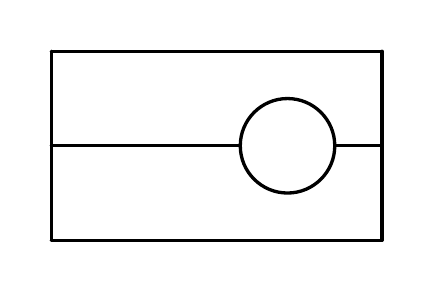
\begin{tikzpicture}[scale=0.3,line cap=round,line join=round,>=triangle 45,x=1.0cm,y=1.0cm]
\clip(-3,-3) rectangle (13,7);
\draw [line width=1.2pt] (-2,6)-- (-2,-2);
\draw [line width=1.2pt] (-2,-2)-- (12,-2);
\draw [line width=1.2pt] (12,-2)-- (12,6);
\draw [line width=1.2pt] (12,6)-- (-2,6);
\draw [line width=1.2pt] (8,2) circle (2cm);
\draw [line width=1.2pt] (10,2)-- (12,2);
\draw [line width=1.2pt] (6,2)-- (-2,2);
\end{tikzpicture}
\end{minipage}

\begin{oefening}
Op het {\em todo}-lijstje van Jef staan zeven dringende taken en vier niet dringende.
\begin{enumerate}[(a)]
  \item Hij neemt zijn agenda en noteert op elke dag van van volgende week één van de dringende taken. Op hoeveel manieren kan hij zijn agenda voor die week invullen?
  \item Als hij geen rekening houdt met de dringendheid van de taken, op hoeveel manieren kan hij dan zijn werk verdelen over de volgende week? Hij wil nog steeds maar één taak per dag uitvoeren.
  \item Eén van de dringende zaken wil hij per se op zaterdag uitvoeren en één van de niet dringende op zondag. Op hoeveel manieren kan hij nu zijn agenda invullen als hij weer uit de volledige lijst kiest?
\end{enumerate}
\end{oefening}

\begin{oefening}
Aan een paardenkoers nemen 8 paarden deel. Er wordt gevraagd de eerste 4 paarden in de juiste volgorde te geven. Hoeveel van dergelijke voorspellingen zijn er mogelijk?
\end{oefening}

\begin{oefening}
Een jeugdgroep telt 10 leden en wil een bestuur kiezen bestaande uit een voorzitter, een ondervoorzitter, een secretaris en een penningmeester. Hoeveel verschillende bestuurslichamen kunnen er verkozen worden?
\end{oefening}

\begin{oefening}
Op een boekenrek moeten 3 werken over wiskunde en 4 romans gerangschikt worden. We beschikken daartoe over 5 wiskundeboeken en over 6 romans. Op hoeveel manieren kunnen we de boeken rangschikken als ons opgelegd wordt de wiskundeboeken vooraan te plaatsen?
\end{oefening}

\begin{oefening}
Met de cijfers $1, 2, 3, \ldots, 9$ vormen we getallen van $6$ verschillende cijfers.
\begin{enumerate}[(a)]
  \item Hoeveel dergelijke getallen zijn er?
  \item Hoeveel ervan beginnen met 1?
  \item Hoeveel ervan beginnen niet met 2?
  \item Hoeveel ervan beginnen met 83?
  \item Hoeveel ervan beginnen niet met 123?
  \item Hoeveel ervan bevatten het cijfer 7?
  \item Hoeveel ervan bevatten wel 4, maar niet 5?
  \item Hoeveel ervan bevatten noch 8, noch 9?
  \item Hoeveel ervan bevatten de cijfers 4 en 5?
\end{enumerate}
\end{oefening}

\begin{oefening}
Op hoeveel manieren kan ik 10 boeken op een plank rangschikken als een bepaald boek op de eerste plaats moet staan?
\end{oefening}

\begin{oefening}
Op hoeveel manieren kunnen we 4 jongens en 3 meisjes op een rij zetten als in geen geval 2 jongens naast elkaar mogen staan?
\end{oefening}

\begin{oefening}
\begin{enumerate}[(a)]
  \item Schrijf alle permutaties van de elementen $a,b,c,d$ op.
  \item Schrijf alle permutaties van de elementen $a,b,c,c$ op.
\end{enumerate}
\end{oefening}

\begin{oefening}
We moeten vijf verschillende prijzen verloten onder de nummers 1 tot en met 100.
Het eerste getrokken nummer krijgt de mooiste prijs, enz. Na het trekken wordt het
nummer verwijderd (We spreken van trekken zonder terugleggen.)
Geef het aantal mogelijke trekkingen.
\end{oefening}

\begin{oefening}
Een vlag moet bestaan uit 2 verticale banen van verschillend gekleurde stof.
Men beschikt over 8 kleuren. Hoeveel vlaggen zijn hiermee samen te stellen?
\end{oefening}

\begin{oefening}
Met de cijfers 3, 4, 5, 6, 7, 8 worden getallen van 3 verschillende cijfers gevormd.
\begin{enumerate}[(a)]
  \item Hoeveel dergelijke getallen bestaan er?
  \item Hoeveel van deze getallen eindigen op 5?
\end{enumerate}
\end{oefening}

<<<<<<< Updated upstream
\pagebreak

\section{Herhalingsvariaties}

\subsection{Voorbeeld}

Op hoeveel manieren kunnen vijf, verschillend gekleurde bollen in de vakjes $a$, $b$ en $c$ geplaatst worden? In elk vakje is er plaats voor méér dan één bol.

\begin{oefening}
Definieer de verzameling van bollen en verzameling vakjes voor het probleem:
\begin{itemize}
  \item \arule{4cm}:  $A =$ \arulefill%\{b_1 , b_2 , b_3 , b_4 , b_5 \}$ met $\#A = 5$
  \item \arule{4cm}: $B =$\arulefill %\{a, b, c\}$ met $\#B = 3$.
\end{itemize}
\end{oefening}

\begin{oefening}
De manier van bollen plaatsen is een samengestelde beslissing. Uit hoeveel deelbeslissingen bestaat deze?
\arules{2}
\end{oefening}

\begin{oefening}
Neem de verschillende deelbeslissingen:
\arules{12}
\end{oefening}

\begin{oefening}
Geef een paar verschillende mogelijke plaatsingen.
\arules{3}
\end{oefening}

Deze manier van plaatsen noteren we met behulp van een vijftal, bijvoorbeeld:
$$(a, a, b, c, b)\;.$$
Voor andere keuzen zullen we andere vijftallen vinden: bv: $(b, a, b, a, c)$, $(c, c, c, a, a)$, $(b, a, a, a,
b)$, $(b, b, b, b, b)$ enz.

\begin{oefening}
Geef het vijftal dat je zelf gebruikt hebt als voorbeeld toen je de verschillende deelbeslissingen nam:
\arules{1}
\end{oefening}

Daar er in elk vakje meerdere bollen kunnen liggen kan een vakje herhaald worden.
Elk vijftal is een samengestelde beslissing met herhaling. Wel, zulk vijftal noemen
we een herhalingsvariatie van vijf elementen gekozen uit een totaal van drie elementen.
Het aantal herhalingsvariaties kunnen we nu gemakkelijk vinden als we de productregel gebruiken.
Het aantal herhalingsvariaties van 5 elementen uit 3 elementen schrijven we kort met het nieuwe symbool $\bar{V}^5_3$.

\begin{oefening}
Geef in ons voorbeeld het aantal mogelijke plaatsingen:
\arules{3}
\end{oefening}

\paragraph*{Let op de notatie}
De $\bar{V}$ is het symbool voor het aantal herhalingsvariaties.
Het aantal elementen (vakjes) wordt onderaan als index geschreven. Het aantal
deelbeslissingen (bollen leggen) wordt bovenaan genoteerd.

\pagebreak
\subsection{Formule}

\begin{oefening}
Leid de formule voor het aantal herhalingsvariaties van $k$ elementen gekozen uit $n$ elementen af:
\arules{9}
\end{oefening}

\paragraph*{Herhalingsvariaties}
\begin{mdframed}
Het aantal {\bf herhalingsvariaties van $k$ verschillende elementen gekozen uit $n$ verschillende elementen} noteren we $\bar{V}^k_n$ en er geldt:
$$\bar{V}^k_n=n^k$$
\end{mdframed}

\paragraph*{Belangrijk}
\begin{itemize}
  \item De positie waarin de elementen worden geplaatst is belangrijk, {\bf volgorde is van belang}.
  \item De elementen kunnen meer dan eens op de zelfde positie terecht komen, {\bf herhaling is mogelijk}.
\end{itemize}

\subsection{Oefeningen}

\begin{oefening}
Aline, Birgit, Celine en Delphine zijn leerlingen uit eenzelfde klas die alle vier in de maand april verjaren.
\begin{enumerate}[(a)]
  \item Hoeveel mogelijkheden zijn er voor hun vier verjaardagen?
  \item Hoeveel mogelijkheden zijn er als je weet dat het vier verschillende data zijn?
  \item Als je weet dat Celine op 10 april jarig is, hoeveel mogelijkheden zijn er dan voor de vier verjaardagen als ze niet noodzakelijk op een verschillende dag moeten verjaren?
\end{enumerate}
\end{oefening}

\begin{oefening}
Met de cijfers 1, 2 en 3 worden getallen van 5 cijfers gevormd.
\begin{enumerate}[(a)]
  \item Hoeveel getallen zijn er?
  \item Hoeveel van die getallen zijn even?
  \item Hoeveel van die getallen bevatten geen cijfer 1?
  \item Hoeveel van die getallen bestaan uit 5 verschillende cijfers?
  \item Welk getal staat op de vijfde plaats als je alle getallen van klein naar groot rangschikt?
  \item Bereken de som van alle getallen.
\end{enumerate}
\end{oefening}

\begin{oefening}
Bij een gezelschapsspel moeten we 4 gekleurde staafjes in een zekere volgorde naast elkaar zetten. Hoeveel mogelijkheden zijn er als we over 6 kleuren beschikken? Je mag er van uit gaan dat elk kleur voldoende voorradig is.
\end{oefening}

\begin{oefening}
Een leraar moet zijn leerlingen evalueren door achter hun naam één van de vermeldingen uitstekend (U), zeer goed (ZG), goed (G), voldoende (V), niet voldoende (NV) of slecht (S) te schrijven. Op hoeveel manieren kan hij een lijst van 12 leerlingen invullen?
\end{oefening}

\begin{oefening}
Van 1962 tot 1971 hadden kentekenplaten twee aaneengeschakelde letters en daarna 3 cijfers in willekeurige volgorde. Hoeveel mogelijke nummerplaten konden ze toen maken?
\begin{center}
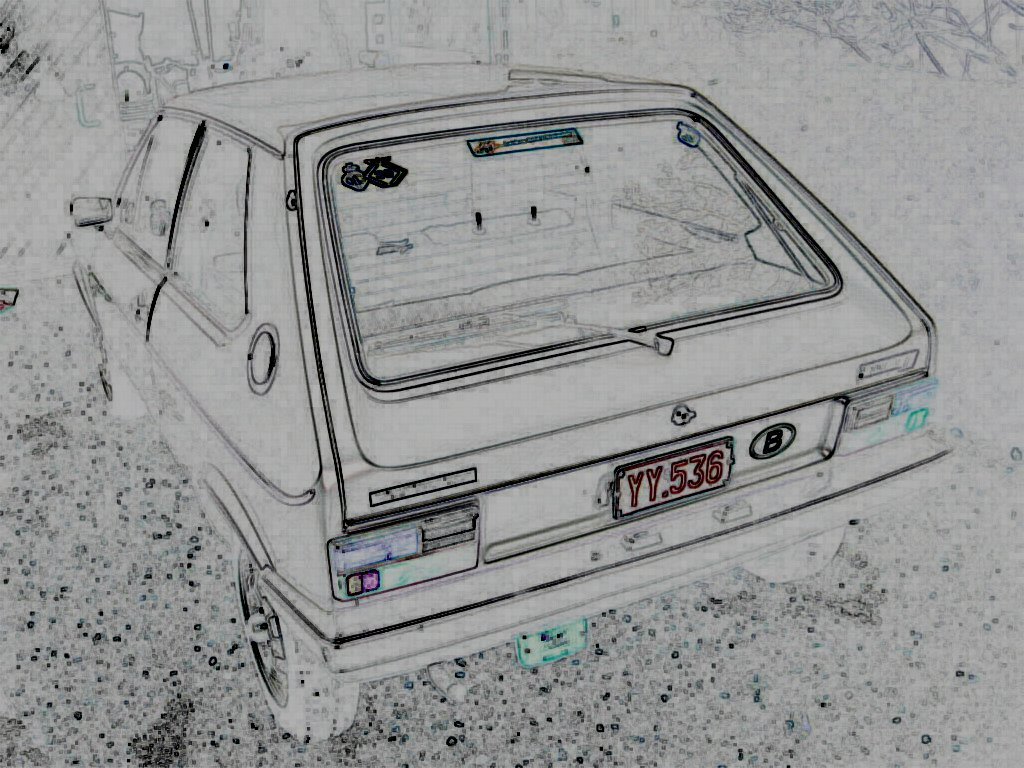
\includegraphics[width=0.5\textwidth]{YY536}
\end{center}
\end{oefening}

\begin{oefening}
We moeten 5 verschillende prijzen verloten onder de nummers 1 tot en met 100.
Na de trekking wordt elk nummer teruggelegd. Geef het aantal mogelijke
trekkingen.
\end{oefening}

\begin{oefening}
Op hoeveel manieren kunnen in een gezin met acht kinderen, de jongens en de
meisjes elkaar opvolgen ?
\end{oefening}

\begin{oefening}
Hoeveel getallen van 4 cijfers kan men vormen met de oneven cijfers ?
\end{oefening}

\begin{oefening}
Schrijf alle herhalingsvariaties op van de elementen a, b en c, twee aan twee
genomen.
Controleer het aantal.
\end{oefening}

\begin{oefening}
Op hoeveel manieren kunnen we een voetbalpronostiek invullen als er 13
wedstrijden worden gespeeld ?
\end{oefening}

\begin{oefening}
Hoeveel “woorden” kunnen we vormen met de letters \verb#a, b, ..., k#. Elk woord
bestaat uit drie letters.
\end{oefening}

\begin{oefening}
Belgische nummerplaten bestaan uit 3 letters en 3 cijfers, bijvoorbeeld \verb#ABA 123#. De letters \verb#I# en de \verb#O# worden niet gebruikt, wegens overeenkomsten met de 1 en de 0. Hoeveel mogelijkheden zijn er om nummerplaten samen te stellen.
\end{oefening}

\begin{oefening} % opmerking, geen herhalingsvariatie!
De fanfare kiest een nieuw bestuur. Uit de 20 leden wordt één directeur, één onderdirecteur en één secretaris gekozen. Op hoeveel manieren kan dit?
\end{oefening}

\begin{oefening} % moeilijk
Hoeveel getallen bestaande uit 3 cijfers kunnen gemaakt worden met 3 vieren, 4 tweeën en 2 drieën.
\end{oefening}

\begin{oefening}
Iedereen weet dat een trol 12 tanden heeft, 6 in elke kaak. Ooit was er eens een leger van 5000 trollen die een draak aanviel. Na het gevecht merkten de overlevende trollen dat geen twee van hun nog de zelfde verzameling tanden had (geen één trol had nog tanden op dezelfde plaats als een andere trol). Hoeveel trollen zijn er tijdens het gevecht tegen de draak op zijn minst gestorven?
\end{oefening}

\pagebreak
\section{n-faculteit}

\subsection{Definitie}

\paragraph*{n-faculteit}
\begin{mdframed}
\begin{align*}
\forall n \in \mathbb{N}\backslash\{0,1\}: n!&=n\cdot(n-1)\cdot(n-2)\cdot \cdots \cdot 3\cdot2\cdot1\\
                                           1!&=1\\
                                           0!&=1\\
\end{align*}
\end{mdframed}

\subsection{Berekenen met behulp van het rekentoetstel}

De toets voor $n$-faculteit bevindt zich boven het rechter haakje. Om bijvoorbeeld $24!$ uit te rekenen toetsen we
$$24 \zrm{SHIFT} \zrm{x!} \zrm{EXE}\;.$$

We krijgen een heel groot getal $6.204484017\EE{23}$ of voluit $620448401733239439360000$.

\subsection{Eigenschap}

\begin{oefening}
Bereken zonder \zrm{ZRM}
\begin{enumerate}[(a)]
  \item $2!=$\arulefill
  \item $3!=$\arulefill\arules{1}
  \item $4!=$\arulefill\arules{1}
  \item $5!=$\arulefill\arules{1}
\end{enumerate}
\end{oefening}


\begin{oefening}
Als je weet dat
$$9!=362880\;.$$
Aan wat is dan $10!$ gelijk? Gebruik geen \zrm{ZRM}.
\end{oefening}

\paragraph*{Eigenschap van de n-faculteit}
\begin{mdframed}
\begin{align*}
  (n+1)!&=(n+1)n!\\
  n!&=n(n-1)!\\
\end{align*}
\end{mdframed}

\begin{oefening}
Bereken zonder \zrm{ZRM}:
\begin{multicols}{3}
\begin{enumerate}[(a)]
  \itemsep0.7em
  \item $\dfrac{17!}{14!}$
  \item $\dfrac{10!}{7!}$
  \item $\dfrac{11!}{8!}$
  \item $\dfrac{8!}{10!}$
  \item $\dfrac{3!\cdot 7!}{10!}$
  \item $\dfrac{12!-10!}{9!}$
\end{enumerate}
\end{multicols}
\end{oefening}

\begin{oefening}
Vereenvoudig:
\begin{multicols}{2}
\begin{enumerate}[(a)]
  \itemsep0.7em
  \item $\dfrac{(n+1)!}{n!}$
  \item $\dfrac{(n-1)!}{n!}$
  \item $\dfrac{n!}{(n+1)!}$
  \item $\dfrac{(n+1)!}{(n-2)!}$
  \item $\dfrac{(n+2)!}{n!}$
  \item $\dfrac{(2n+2)!}{2n!}$
  \item $\dfrac{(n+1)!}{n!}-\dfrac{n!}{(n-1)!}$
  \item $\dfrac{(n+1)!}{(n-1)!}-\dfrac{n!}{(n-2)!}$
\end{enumerate}
\end{multicols}
\end{oefening}

\begin{oefening}
Als je weet dat het getal $99!$ uit 156 cijfers bestaat, uit hoeveel cijfers bestaat dan het getal $100!$
\end{oefening}

\subsection{Formule voor $V^k_n$ met behulp van faculteiten}

\begin{oefening}
Bereken $V^3_7$ door gebruik te maken van faculteiten.
\arules{5}
\end{oefening}

\begin{oefening}
Stel algemeen de formule op van $V^k_n$ door gebruik te maken van faculteiten.
\arules{6}
\end{oefening}

\paragraph*{Variaties} (formule m.b.v. faculteiten)
\begin{mdframed}
$$V^k_n=\dfrac{n!}{(n-k)!}$$
\end{mdframed}

\begin{oefening}
Om het aantal variaties van 20 elementen uit 21 elementen te berekenen hebben we twee formules:\\
\begin{itemize}
  \itemsep1em
  \item $\displaystyle V^{20}_{24}=21\cdot20\cdot19\cdot18\cdot\;\cdots\;\cdot(24-20+1)$
  \item $\displaystyle V^{20}_{24}=\dfrac{24!}{(24-20)!}$
\end{itemize}
\begin{enumerate}[(a)]
  \item Bereken op beide manieren het aantal variaties. Welke methode verkies je in dit geval?
  \item Doe hetzelfde voor het aantal variaties van 3 elementen uit 10 elementen. Welke methode verkies je in dit geval?
  \item Welke methode zou je kiezen als je het aantal variaties van 100 elementen uit 1000 elementen zou moeten berekenen? Het is niet nodig om dit te proberen, hiervoor is speciale software nodig want onze rekenmachines kunnen niet met zulke grote getallen overweg.
\end{enumerate}
\end{oefening}

\pagebreak
\section{Driehoek van Pascal}

\subsection{Voorbeeld}

Beschouw het stratenplan van New York:
\begin{center}
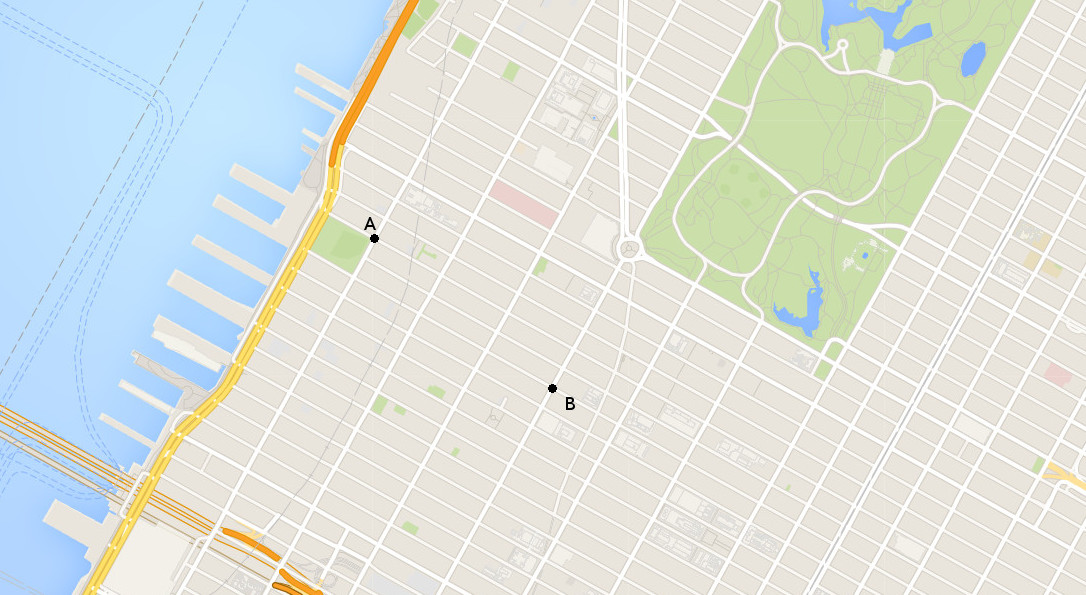
\includegraphics[width=0.8\textwidth]{NY_grid}
\end{center}

We wensen de kortste weg te nemen van $A$ naar $B$. Als we dit plan goed bestuderen merken we dat er meer dan één kortste weg van $A$ naar $B$ is. Hoeveel kortste wegen zijn er?

\begin{oefening}\mbox{}
\begin{enumerate}[(a)]
  \item Stel het stukje stratenplan waarin we geïnteresseerd zijn schematisch voor en gebruik voor een stukje horizontale weg de letter $H$ en voor een stukje verticale weg de letter $V$.
\ruitjes{4cm}
  \item Neem een kleur en duid de weg $HVHHV$ aan.
  \item Geef gecodeerd nog twee andere mogelijke kortste wegen van $A$ naar $B$.
  \arules{1}
  \item Beschrijf het uiterlijk van een code die aan de kortste weg voldoet.
  \arules{2}
\end{enumerate}
\end{oefening}

Als we dus het aantal codes vinden, dan vinden we ook het aantal mogelijke kortste wegen. In de wiskunde zullen we vaak een moeilijk probleem oplossen door voor het probleem een equivalent probleem te vinden dat eenvoudiger te beschrijven is.

\subsubsection{Tellen met behulp van een boomdiagram}

\begin{oefening}
Tel het aantal mogelijke codes (en dus ook het aantal mogelijke kortste wegen) met behulp van een boomdiagram.\\

\vspace*{5cm}
start
\vspace*{5cm}

Er zijn dus \arule{3cm} mogelijke codes met 3$H$'s en 2$V$'s. We weten nu dus dat er \arule{3cm} wegen zijn van $A$ naar $B$.
\end{oefening}

Indien $A$ en $B$ verder van elkaar verwijderd zijn, dan wordt dit snel veel ingewikkelder. We zoeken dus een andere manier.

\pagebreak
\subsubsection{Tellen met behulp van een wegenrooster}

\begin{oefening}\mbox{}\\
\begin{multicols}{2}
\begin{center}
\begin{tikzpicture}[line cap=round,line join=round,>=triangle 45,x=1.0cm,y=1.0cm]
\draw (0,0) -- (6,0);
\draw (0,1) -- (6,1);
\draw (0,2) -- (6,2);
\draw (0,0) -- (0,2);
\draw (2,0) -- (2,2);
\draw (4,0) -- (4,2);
\draw (6,0) -- (6,2);
\fill (0,2) circle (1.8pt);
\draw (-0.3,2.3) node {$A$};
\fill  (6,0) circle (1.8pt);
\draw (6.3,0.3) node {$B$};
\end{tikzpicture}
\end{center}  

Duid hiernaast in elke knoop het aantal kortste wegen van $A$ naar die knoop aan. Je moet hiervoor slim gebruik maken van reeds berekende resultaten.
\end{multicols}
Dit wordt tellen via een wegenrooster genoemd. Hoeveel kortste wegen zijn er van $A$ naar $B$?
\arules{1}
\end{oefening}

\subsubsection{Tellen met behulp van een formule}

\begin{oefening}
We moeten een code van 5 plaatsten vullen. Op twee van die vijf plaatsen komt de letter $V$. Je weet dan onmiddellijk waar de $H$'s moeten komen, dit kan je dus negeren. Zoek een formule om die twee $V$'s op vijf posities te plaatsen.
\arules{4}
\end{oefening}

\begin{oefening}
We moeten een code van 5 plaatsten vullen. Op drie van die vijf plaatsen komt de letter $H$. Je weet dan onmiddellijk waar de $V$'s moeten komen, dit kan je dus negeren. Zoek een formule om die drie $H$'s op vijf posities te plaatsen.
\arules{4}
\end{oefening}

\begin{oefening}
Geef zelf een algemene formule om te bepalen hoeveel codes met $n$ plaatsen, waarvan er $k$ worden ingenomen door een eerste symbool en waarbij er $n-k$ worden ingenomen door een tweede symbool, er zijn.
\arules{4}
\end{oefening}

\begin{oefening}
Beschouw het volgende wegenrooster met de locatie van Marieke en Jan en daarbinnen ook een moeras.
\begin{center}
\definecolor{uququq}{rgb}{0.25,0.25,0.25}
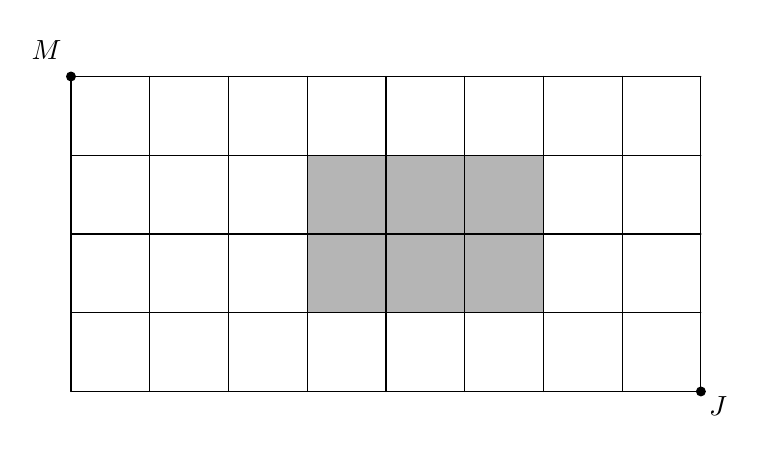
\begin{tikzpicture}[line cap=round,line join=round,>=triangle 45,x=1.0cm,y=1.0cm]
\clip(1.45,1.41) rectangle (10.52,6.62);
\fill[line width=0.4pt,fill=black,fill opacity=0.29] (8,3) -- (5,3) -- (5,5) -- (8,5) -- cycle;
\draw [domain=2:10] plot(\x,{(--2-0*\x)/1});
\draw [domain=2:10] plot(\x,{(--6-0*\x)/2});
\draw [domain=2:10] plot(\x,{(--8-0*\x)/2});
\draw [domain=2:10] plot(\x,{(--10-0*\x)/2});
\draw [domain=2:10] plot(\x,{(--12-0*\x)/2});
\draw (2,2) -- (2,6);
\draw (3,2) -- (3,6);
\draw (4,2) -- (4,6);
\draw (5,2) -- (5,6);
\draw (6,2) -- (6,6);
\draw (7,2) -- (7,6);
\draw (8,2) -- (8,6);
\draw (9,2) -- (9,6);
\draw (10,2) -- (10,6);
\fill (2,6) circle (1.8pt);
\draw (1.69,6.34) node {$M$};
\fill  (10,2) circle (1.8pt);
\draw (10.22,1.81) node {$J$};
\end{tikzpicture}
\end{center}
\begin{enumerate}[(a)]
  \item Hoeveel wegen zijn er van Marieke naar Jan?
  \item Hoeveel zijn er als ze niet langs het moeras kan wandelen?
\end{enumerate}
\end{oefening}

\begin{oefening}
Beschouw het volgende wegenrooster met de locaties $S$, $V$ en $T$.
\begin{center}
\definecolor{uququq}{rgb}{0.25,0.25,0.25}
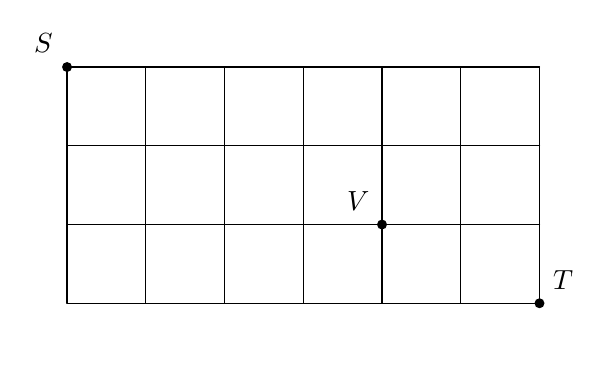
\begin{tikzpicture}[line cap=round,line join=round,>=triangle 45,x=1.0cm,y=1.0cm]
\clip(-0.5,-0.5) rectangle (6.5,3.5);
\draw (0,0) -- (6,0);
\draw (0,1) -- (6,1);
\draw (0,2) -- (6,2);
\draw (0,3) -- (6,3);
\draw (0,0) -- (0,3);
\draw (1,0) -- (1,3);
\draw (2,0) -- (2,3);
\draw (3,0) -- (3,3);
\draw (4,0) -- (4,3);
\draw (5,0) -- (5,3);
\draw (6,0) -- (6,3);
\fill (0,3) circle (1.8pt);
\draw (-0.3,3.3) node {$S$};
\fill  (4,1) circle (1.8pt);
\draw (3.7,1.3) node {$V$};
\fill  (6,0) circle (1.8pt);
\draw (6.3,0.3) node {$T$};
\end{tikzpicture}
\end{center}
\begin{enumerate}[(a)]
  \item Hoeveel wegen zijn er van $S$ naar $T$?
  \item Hoeveel wegen zijn er van $S$ naar $T$ als je via $V$ wilt gaan?
\end{enumerate}
\end{oefening}

\pagebreak
\subsection{Driehoek van Pascal}

\begin{oefening}
Teken een oneindig doorlopend wegenrooster met beginpunt $P$ en waarbij er bij elk kruispunt ten aantal mogelijke kortste wegen wordt genoteerd. Ga ervan uit dat er van $P$ naar $P$ één mogelijke kortste weg is, ter plaatse blijven staan, zet je bij $P$ het getal 1.
\begin{center}
  $P$
\end{center}
\ruitjes{16cm}
\end{oefening}
\begin{mdframed}
De bekomen oneindige naar beneden doorlopende driehoek wordt de {\bf driehoek van Pascal} genoemd.
\end{mdframed}


\begin{oefening}
Beschouw de driehoek van Pascal.
\begin{enumerate}[(a)]
  \item Welke getallen staan er op rij 9?
  \item Welke getallen staan er op rij 10?
  \item Hoeveel getallen staan er op rij $0$, rij $1$, rij $2$, $\ldots$, rij $n$?
  \item Maak de som van de getallen op de opeenvolgende rijen.
\end{enumerate}
\end{oefening}

\begin{oefening}
Op de titelpagina van dit hoofdstuk werd de driehoek van Pascal getekend. Een bepaald soort getallen werd gemarkeerd. Welke? Als we dit doen wordt een nieuw soort wiskundige driehoek geconstrueerd, namelijk de driehoek van Sierpiński. Beschrijf nog één andere manier om deze driehoek te construeren.
\end{oefening}

\subsection{Binomium van Newton}

\begin{oefening}
Vul de tabel aan:\\
\hspace*{-1.5cm}
%\begin{center}
  \begin{tabular}{l|l}
  machten van $(x+y)$ & coëfficiënten\\
  \hline
  $(x+y)^0 = 1$ & 1\\
  $(x+y)^1 = x+y$ & 1\qquad 1\\ 
  $(x+y)^2 = $\arule{3cm} & \arule{3cm}\\
  $(x+y)^3 = $\arule{4cm} & \arule{4cm}\\
  $(x+y)^4 = $\arule{5cm} & \arule{5cm}\\
  $(x+y)^5 = $\arule{6cm} & \arule{6cm}\\
  \vdots & \vdots\\
  $(x+y)^8 = $\arule{8cm} & \arule{8cm}\\
  \end{tabular}
%\end{center}
\end{oefening}

\begin{oefening}
Bereken de coëfficiënten van $(x+y)^4$:
\arules{3}
\end{oefening}

\newpage
Deze formule is dusdanig handig dat we deze coëfficiënten een naam geven, algemeen noemen we dit de {\bf binomiaalcoëfficiënt} van $k$ uit $n$ en noteren

\paragraph*{Binomiaalcoëfficiënten}
\begin{mdframed}
$${k \choose n} = \dfrac{n!}{k!\cdot\left(n-k!\right)}$$
\end{mdframed}

\begin{oefening}
Beschouw opnieuw de vierde macht van $x+y$:
\begin{align*}
  (x+y)^4 &= x^4 + 4x^3y+6x^2y^2+4xy^3+y^4\\
          &= 1x^4y^0 + 4x^3y^1+6x^2y^2+4x^1y^3+1x^0y^4\\
          &= {4 \choose 0}x^4y^0 + {4 \choose 1}x^3y^1+{4 \choose 2}x^2y^2+{4 \choose 3}x^1y^3+{4 \choose 4}x^0y^4\\
\end{align*}
\begin{enumerate}[(a)]
  \item Bespreek de vorm van elke term:
  \arules{4}
  \item Hoe is de $k$-de term dan te schrijven:
  \arules{3}
  \item Schrijf dan de vierde macht van $x+y$ kort door gebruik te maken van het sommatiesymbool $\displaystyle\Sigma$:
  \arules{3}
\end{enumerate}
\end{oefening}

\begin{oefening}
Schrijf de zevende macht van $x+y$:
\arules{3}
\end{oefening}

\pagebreak
We krijgen algemeen
\paragraph{Binomium van Newton}
\begin{mdframed}
Voor $a,b\in\mathbb{R}$ en $n\in\mathbb{N}_0$ geldt:
$$(a+b)^n=\sum^n_{k=0}{n \choose k}a^{n-k}b^k$$
\end{mdframed}

Bijvoorbeeld:
\begin{align*}\displaystyle
  (x-1)^4 &= \sum^4_{k=0}{4 \choose k}x^{4-k}(-1)^k\\
          &= {4 \choose 0}x^4(-1)^0 + {4 \choose 1}x^3(-1)^1+{4 \choose 2}x^2(-1)^2+{4 \choose 3}x^1(-1)^3+{4 \choose 4}x^0(-1)^4\\
          &=x^4-4x^3+6x^2-4x+1
\end{align*}


\begin{oefening}
Werk uit:
%\begin{multicols}{3}
\begin{enumerate}[(a)]
  \item $\left(x-2y\right)^4$
  \item $\left(a^2-c\right)^8$
  \item $\left(\sqrt{5}-1\right)^4$
  \item $\left(x-\dfrac{1}{x}\right)^6$
\end{enumerate}
%\end{multicols}
\end{oefening}

\begin{oefening}
Bereken:
\begin{enumerate}[(a)]
  \item de 6de term van $\left(1-\dfrac{1}{b}\right)^9$
  \item de 21ste term van $\left(x^2-\dfrac{a}{x}\right)^{24}$
\end{enumerate}
\end{oefening}

\begin{oefening}
Bereken zonder \zrm{ZRM} $$\left(\sqrt{2}+1\right)^5+\left(\sqrt{2}-1\right)^5$$
\end{oefening}

\pagebreak
\subsection{Extra Oefeningen}  % mathcentre

\begin{oefening}
Werk uit m.b.v. binomium van Newton:
\begin{multicols}{3}
\begin{enumerate}[(a)]
  \item $\left(1+3x\right)^2$
  \item $\left(2+x\right)^3$
  \item $\left(1-x\right)^3$
  \item $\left(1-5x\right)^5$
  \item $\left(x+6\right)^3$
  \item $\left(a-b\right)^7$
  \item $\left(1+\dfrac{3}{a}\right)^4$
  \item $\left(x-\dfrac{1}{x}\right)^6$
\end{enumerate}
\end{multicols}
\end{oefening}

\begin{oefening}
Gebruik het binomium van Newton om de eerste drie termen in dalende macht van $x$ te vinden voor $\left(1-\dfrac{x}{2}\right)^8$.
\end{oefening}

\begin{oefening}
Zoek de coëfficiënt van $x^5$ in de ontwikkeling van $\left(1+4x\right)^9$.
\end{oefening}

\begin{oefening}
Zoek in de ontwikkeling van $\left(1-x\right)^8$ de coëfficiënt die hoort bij $x^7$.
\end{oefening}

\begin{oefening}
Zoek de eerste vier termen in de ontwikkeling van $\left(2+\dfrac{x}{3}\right)^{12}$.
\end{oefening}

\pagebreak
\section{Combinaties}

\subsection{Voorbeeld}

Op hoeveel manieren kunnen twee identieke bollen in vijf verschillende vakjes geplaatst worden? In elk vakje mag hoogstens één bol voorkomen.

We definiëren:
\begin{itemize}
  \item De bollen zijn identiek, we duiden één bol aan met de letter $B$
  \item De verzameling vakjes = $\{a, b, c, d, e\}$
\end{itemize}

We moeten twee gelijke bollen in vijf vakjes leggen. Dit is hetzelfde als: we moeten de twee bollen tegelijkertijd in de bakjes leggen. Vermits de 2 bollen identiek zijn heeft alléén het vakje belang waarin een bol ligt. De bol zelf speelt geen rol.

\begin{oefening}
Teken een mogelijke plaatsing van de bollen:
\arules{2}
\end{oefening}

Elke plaatsing zouden we als een tweetal $(a, c)$ kunnen noteren. Maar elk tweetal, waarin dezelfde vakjes voorkomen zoals $(a, c)$ en $(c, a)$ stelt eenzelfde plaatsing voor.

De volgorde waarin de vakjes opgesomd worden heeft geen belang. We spreken nu
af om de plaatsing te noteren als een verzameling waarin de elementen in
alfabetische volgorde worden geschreven. De hierboven voorgestelde plaatsing
wordt dan : $\{a, c\}$ en is een deelverzameling van de gegeven verzameling vakjes $\{a, b, c, d, e\}$.

Daar er bovendien in elk vakje hoogstens één bol ligt wordt geen enkel vakje
herhaald. In een verzameling wordt óók geen element herhaald. Wel, de
deelverzameling $\{a, c\}$, noemt men nu een combinatie zonder herhaling, kortweg combinatie, van 2 elementen gekozen uit 5 elementen.
Het aantal van zulke combinaties stellen we nu voor door het symbool $C^2_5$ en kunnen we als volgt bepalen:

\begin{oefening}
Codeer het gegeven probleem als volgt: We kiezen 5 plaatsen, 2 ervan moeten gevuld worden met de letter $B$ van bol plaatsen, de overige drie moeten gevuld worden met de letter $L$ van leeg laten. Los dit probleem nu op met behulp van een wegenrooster.
\ruitjes{4cm}
\end{oefening}

Eenvoudiger is om onmiddellijk de formule te gebruiken:
$$C^2_5=\dfrac{5!}{2!\cdot (5-2)!}$$

\begin{oefening}
Maak voorgaande berekening. Met andere woorden, op hoeveel manieren kunnen twee identieke bollen in vijf verschillende vakjes geplaatst worden als in één vakje hoogstens één bol mag voorkomen?
\arules{2}
\end{oefening}

Let op de notatie : De $C$ is het symbool voor het aantal combinaties zonder
herhaling. Het aantal vakjes (elementen) waarover je beschikt wordt als index
genoteerd. Het aantal te vullen vakjes wordt bovenaan genoteerd.

\vspace*{-1cm}
\subsection{Formule}

\paragraph*{Combinaties}
\begin{mdframed}
Het aantal {\bf combinaties van $k$ elementen gekozen uit $n$ elementen} noteren we $C^k_n$ en er geldt:
$$C^k_n=\dfrac{n!}{k!\cdot(n-k)!}$$
\end{mdframed}

\paragraph*{Belangrijk}
\begin{itemize}
  \item Het maakt niet uit in welke volgorde dat de elementen worden gekozen, {\bf volgorde onbelangrijk}.
  \item Elk element kunnen we maar éénmaal kiezen, {\bf herhaling niet toegestaan}.
\end{itemize}

\subsection{Oefeningen}

\begin{oefening}
Voor het voetbalteam van de school stellen zich 19 jongens kandidaat.
\begin{enumerate}[(a)]
  \item Hoeveel elftallen kan de coach hiermee vormen?
  \item Bij het samenstellen van de ploeg voor een belangrijke wedstrijd wil de coach zijn vijf beste spelers zeker opstellen en zijn drie zwakste niet. Hoeveel ploegen kan hij nu vormen?
\end{enumerate}
\end{oefening}

\begin{oefening}
Een Belgische delegatie bestaat uit 7 Vlamingen en 5 Walen.
\begin{enumerate}[(a)]
  \item Hoeveel groepjes van 6 personen kan je hiermee vormen?
  \item Hoeveel groepjes bestaan uit 3 Vlamingen en 3 Walen?
\end{enumerate}
\end{oefening}

\begin{oefening}
Een firma heeft twee bedienden nodig (die hetzelfde werk moeten verrichten). Er zijn acht sollicitanten. Op hoeveel manieren kan de directie haar keuze bepalen?
\end{oefening}

\begin{oefening}
In een firma werken 15 arbeiders en 10 bedienden. Op hoeveel verschillende manieren kunnen we een comité samenstellen dat uit 3 arbeiders en 2 bedienden bestaat?
\end{oefening}

\begin{oefening}
Herinner je nog deze oefening uit het hoofdstuk van variaties:

{\em Op een boekenrek moeten 3 werken over wiskunde en 4 romans gerangschikt worden. We beschikken daartoe over 5 wiskundeboeken en over 6 romans. Op hoeveel manieren kunnen we de boeken rangschikken als ons opgelegd wordt de wiskundeboeken vooraan te plaatsen?}

Los deze nu opnieuw op, maar het is nu wel niet meer nodig om de wiskundeboeken vooraan te plaatsen.
\end{oefening}

\begin{oefening}
De bibliotheek bezit 15 verschillende werken van een schrijver die net de Nobelprijs voor literatuur heeft gekregen. Naar aanleiding daarvan worden 10 werken op een speciale tafel tentoongesteld. Hoeveel keuzemogelijkheden heeft de bibliothecaris?
\end{oefening}

\begin{oefening}
Bij vele spelletjes met een stel van 52 kaarten krijg je 13 kaarten.
\begin{enumerate}[(a)]
  \item Hoeveel mogelijkheden zijn er om uit 52 kaarten er 13 te trekken (zonder kaarten terug te leggen)?
  \item In hoeveel van die gevallen heb je geen enkele aas?
  \item Hoeveel mogelijkheden zijn er met schoppen aas?
  \item Hoeveel mogelijkheden zijn er met 4 azen?
  \item Hoeveel mogelijkheden zijn er met precies 3 azen?
  \item In hoeveel van die mogelijkheden heb je alle harten?
  \item Hoeveel mogelijkheden zijn er met 9 harten en 4 klaveren?
\end{enumerate}
\end{oefening}

\begin{oefening}
Bepaal voor de volgende problemen of het een combinatie of een variatie is.
\begin{enumerate}[(a)]
  \item Uit een klas worden zes leerlingen gekozen om een volleybalteam te vormen.
  \item Bij een verloting zijn drie prijzen te verdienen: een fiets, een fles wijn en een taart.
  \item Van 100 leraren van een school komen er vijf naar het schoolfeest.
  \item In een klas worden vijf kaartjes verloot voor een concert.
  \item Uit de muziek top 10 van vorige week stel je een persoonlijke top drie samen.
  \item Een vereniging kiest een voorzitter, een secretaris en een penningmeester.
  \item Een bondscoach kiest 24 spelers voor de selectie die hij meeneemt naar het WK.
\end{enumerate}
\end{oefening}

\begin{oefening}
Uit een selectie van 19 personen wordt een spelersraad van 6 spelers samengesteld. Hoeveel spelersraden zijn er mogelijk?
\end{oefening}

\begin{oefening}
Uit de spelersraad van 6 personen wordt een bestuur gekozen dat bestaat uit een voorzitter, een secretaris en een penningmeester. Hoeveel besturen zijn er mogelijk?
\end{oefening}

\begin{oefening}
Uit de selectie van 19 personen wordt een feestcommissie gekozen die uit 5 personen bestaat. Hoeveel feestcommissies zijn er mogelijk?
\end{oefening}

\begin{oefening}
In de mediatheek staat 14 CD's met klassieke muziek en 12 CD's met popmuziek. Margo kiest 5 CD's met klassieke muziek. Hoeveel mogelijkheden zijn er?
\end{oefening}

\begin{oefening}
Joni gooit 13 keer met een geldstuk. Telkens noteert hij K(op) en M(unt). Zo ontstaat een serie met 13 letters K en M.
\begin{enumerate}[(a)]
  \item Hoeveel series zijn er met 11 keer K?
  \item Hoeveel series zijn er met 9 keer een M?
  \item Hoeveel series zijn er die met K beginnen en met M eindigen?
\end{enumerate}
\end{oefening}

\pagebreak
\section{Herhalingscombinaties}

\subsection{Voorbeeld}

Marieke wordt 5 jaar. Voor haar verjaardagsfeestje hangt de vader 5 ballonnen aan de voordeur. Hij heeft ballonnen in 4 kleuren: blauwe (B), gele (G), rode (R) en witte (W). Marieke mag de kleuren kiezen, een mengeling van kleuren of zelfs allemaal in één kleur. Op hoeveel manieren kan ze dit doen?

\paragraph*{Belangrijk}
\begin{itemize}
  \item Het maakt niet uit in welke volgorde dat de ballonnen worden gekozen, {\bf volgorde onbelangrijk}.
  \item Ze kan een kleur van ballon opnieuw kiezen, {\bf herhaling toegestaan}.
\end{itemize}

We tellen het aantal mogelijkheden.

Hou voor elk kleur voldoende ruimte:

\verb# B | G | R | W #

Op deze manier worden de kleuren van elkaar gescheiden door een eerste symbool \verb#|#

We nemen een tweede symbool \verb#*# om de gekozen kleur voor te stellen.

\begin{oefening}
Stel de volgende keuzes voor:
\begin{enumerate}[(a)]
  \item drie blauwe ballonnen, één groene, één rode: \arulefill
  \item Marieke kiest allemaal witte ballonnen: \arulefill
  \item twee blauwe, één witte en de rest ook blauw: \arulefill
\end{enumerate}
\end{oefening}

Merk nu op dat elke code bestaat uit 8 plaatsen, waaruit we er 5 moeten kiezen om een \verb#*# te zetten. We vinden dus het aantal mogelijkheden met een combinatie: $C^5_8=\dfrac{8!}{5!3!}=56$

We noemen het aantal keuzemogelijkheden het aantal {\bf herhalingscombinaties van 5 uit 4}, ja want we kiezen 5 ballonnen en voor elke ballon hebben we vier kleuren om uit te kiezen. We nemen dus 5 beslissingen en voor elke beslissing hebben we vier keuzes. We noteren dit kort als
$$\bar{C}^5_4=C^5_8=56$$

\pagebreak
\subsection{Algemeen}

\paragraph*{Herhalingscombinaties}
\begin{mdframed}
Het aantal {\bf herhalingscombinaties van $k$ elementen gekozen uit $n$ verschillende elementen} noteren we $\bar{C}^k_n$ en er geldt:
$$\bar{C}^k_n=C^k_{n+k-1}$$
\end{mdframed}

\paragraph*{Belangrijk}
\begin{itemize}
  \item Het maakt niet uit in welke volgorde dat de elementen worden gekozen, {\bf volgorde onbelangrijk}.
  \item Elk element kunnen we meerdere keren opnieuw kiezen, {\bf herhaling toegestaan}.
\end{itemize}

\paragraph*{Opmerking}
In de formule kan $k$, het aantal elementen dat wordt gekozen, groter zijn dan $n$, het aantal elementen waaruit we kiezen.


\subsection{Oefeningen}

\begin{oefening}
Een bloemist maakt bloemstukjes waarin hij telkens 11 voorjaarsbloemen verwerkt. Hij beschikt over tulpen (witte, gele en oranje), narcissen (witte en gele) en anemonen (witte en paarse).
\begin{enumerate}[(a)]
  \item Hoeveel verschillende composities kan hij maken?
  \item Hoeveel composities bevatten geen witte bloemen?
  \item Hoeveel composities bevatten enkel tulpen?
\end{enumerate}
\end{oefening}

\begin{oefening}
In het casino wordt een gokspel gespeeld waarbij je jetons op een speelbord met zes velden mag plaatsen. Je mag de jetons verdelen zoals je wilt.
\begin{enumerate}[(a)]
  \item Hoeveel verdelingen van de jetons zijn er mogelijk als je er 5 inzet?
  \item Hoeveel verdelingen van de jetons zijn er mogelijk als je er 10 inzet?
\end{enumerate}
\end{oefening}

\begin{oefening}
Er worden doosjes gevuld met pralines. Er is een voorraad pralines gemaakt in 4 soorten: pure chocolade, melkchocolade, witte chocolade en gemengd. Van elke soort zijn er 10 verschillende vormen en vullingen.
\begin{enumerate}[(a)]
  \item Hoeveel mogelijkheden zijn er als je van elke soort chocolade 5 pralines van verschillende vormen en vullingen in het doosje steekt?
  \item Hoeveel mogelijkheden zijn er als je van elke soort chocolade 5 pralines in het doosje steekt zonder op de vorm en de vulling te letten?
\end{enumerate}
\end{oefening}

\section{Anagrammen}

\subsection{Voorbeeld}

Hoeveel anagrammen zijn er van het woord \verb#ANANAS#?

We moeten dus zes letters rangschikken, waarvan
\begin{itemize}
  \item 3 keer de letter \verb#A#
  \item 2 keer de letter \verb#N#
  \item 1 keer de letter \verb#S#
\end{itemize}

\begin{enumerate}
  \item Veronderstel dat de zes letters allemaal verschillend zijn:\\
  $$\Rightarrow \#=6\cdot5\cdot4\cdot3\cdot2\cdot1=720=6!=P_6$$
  \item We hebben echter teveel geteld, om dit in te zien noteren we de letters als volgt:
  $$A_1N_1A_2N_2A_3S_1$$
  We tellen nu op hoeveel manieren we éénzelfde anagram kunnen bekomen, bijvoorbeeld \verb#NAANSA#:
  \begin{center}
  \begin{tabular}{ccc}
    $N_1A_1A_2N_2S_1A_3$ & $N_1A_1A_3N_2S_1A_2$ & $N_1A_2A_1N_2S_1A_3$\\
    $N_1A_2A_3N_2S_1A_1$ & $N_1A_3A_1N_2S_1A_2$ & $N_1A_3A_3N_2S_1A_1$\\
    $N_2A_1A_2N_1S_1A_3$ & $N_2A_1A_3N_1S_1A_2$ & $N_2A_2A_1N_1S_1A_3$\\
    $N_2A_2A_3N_1S_1A_1$ & $N_2A_3A_1N_1S_1A_2$ & $N_2A_3A_3N_1S_1A_1$\\
  \end{tabular}
  \end{center}
  We merken dus op dat we elk uniek anagram op 12 manieren kunnen bekomen:
  \begin{itemize}
    \item \verb#N# neemt 2 plaatsen in, dit kan op $P_2=2!=2$ manieren
    \item \verb#A# neemt 3 plaatsen in, dit kan op $P_3=3!=3\cdot2=6$ manieren
  \end{itemize}
  $$\Rightarrow \#=P_2\cdot P_3=2\cdot6=12$$
  \item Dus het aantal anagrammen van het woord \verb#ANANAS#
  $$=\dfrac{P_6}{P_2\cdot P_3}=\dfrac{6!}{2!\cdot 3!}=\dfrac{720}{12}=60$$
\end{enumerate}

\begin{oefening}
Bepaal het aantal anagrammen van je eigen naam.
\arules{4}
\end{oefening}

\subsection{Algemeen}

We rangschikken $n$ elementen, waarvan
\begin{itemize}
  \item $n_1$ van de eerste soort
  \item $n_2$ van de tweede soort
  \item $n_3$ van de derde soort
  \item $\vdots$
  \item $n_k$ van de $k$-de soort
\end{itemize}
met $n_1+n_2+n_3+\dots+n_k=n$. De bekomen resultaten noemen we {\bf anagrammen}. Het aantal anagrammen wordt gegeven door

\paragraph*{Anagrammen}
\begin{mdframed}
$$P^{n_1,n_2,n_3,\dots,n_k}_n = \dfrac{n!}{n_1!\cdot n_2!\cdot n_3!\cdot \cdots \cdot n_k!}$$
\end{mdframed}

\subsection{Oefeningen}

\vspace*{-0.5cm}
\begin{oefening}
Noteer alle anagrammen van het woord \verb#EEFJE#. Bereken vervolgens het aantal anagrammen met de formule.
\end{oefening}

\begin{oefening}
Noem $V$ de verzameling van alle natuurlijke getallen van 5 cijfers die tweemaal het cijfer 1 en driemaal het cijfer 2 bevatten.
\begin{enumerate}[(a)]
  \item Noteer het aantal elementen van $V$ van klein naar groot.
  \item Bereken het aantal elementen van $V$.
  \item Bereken het aantal getallen van $V$ die even zijn.
\end{enumerate}
\end{oefening}

\begin{oefening}
Bereken het aantal anagrammen van \verb#MISSISSIPPI#.
\end{oefening}

%%%%%%%%%%%%%%%%%%%%%%%%%%%%%%%%%%%%%%%%%%%%%%%%%%%%%%%%%%%%%%%%%%%%%%
\end{document}
























